\documentclass{article}%
\usepackage[T1]{fontenc}%
\usepackage[utf8]{inputenc}%
\usepackage{lmodern}%
\usepackage{textcomp}%
\usepackage{lastpage}%
\usepackage{geometry}%
\geometry{margin=1in}%
\usepackage{ragged2e}%
\usepackage{graphicx}%
%
\title{AutoStatAgent: An Agent-Based System for Automated Data Analysis and LaTeX Report Generation}%
\author{AutoStatAgent System}%
\date{\today}%
\usepackage{float}%
\usepackage{float}%
%
\begin{document}%
\normalsize%
\maketitle%
\section*{Abstract}%
\label{sec:Abstract}%
The project proposes an intelligent agentic system, AutoStatAgent, that automatically performs complete exploratory data analysis (EDA) and statistical testing on any given dataset. By leveraging autonomous agents, the system generates and answers relevant analytics questions, visualizes insights using smart aesthetics, and compiles the results into a professional LaTeX{-}based PDF report. The system democratizes data analytics by allowing users to simply upload a dataset without needing any statistical or programming background.

%
\newpage%
\section{Introduction}%
\label{sec:Introduction}%
Many individuals, especially in academia and business, possess valuable datasets but lack the statistical knowledge or programming skills to derive insights. There is a need for a system that not only analyzes data but also presents results in a readable, interpretable, and publishable format—fully automated.

%
\section{Dataset Overview}%
\label{sec:DatasetOverview}%
\textbf{Column: original\_price}%
 | Type: Unknown | Non{-}missing: 2176.0 | Missing: 0\newline%
\newline%
%
\textbf{Column: markdown\_percentage}%
 | Type: Unknown | Non{-}missing: 2176.0 | Missing: 0\newline%
\newline%
%
\textbf{Column: current\_price}%
 | Type: Unknown | Non{-}missing: 2176.0 | Missing: 0\newline%
\newline%
%
\textbf{Column: stock\_quantity}%
 | Type: Unknown | Non{-}missing: 2176.0 | Missing: 0\newline%
\newline%
%
\textbf{Column: customer\_rating}%
 | Type: Unknown | Non{-}missing: 2176.0 | Missing: 0\newline%
\newline%

%
\section{Questions \& Answers}%
\label{sec:QuestionsAnswers}%
\subsection{Does the strong Spearman correlation (r=0.91) between 'original\_price' and 'current\_price' indicate potential causal or confounding factors worth testing?}%
\label{subsec:DoesthestrongSpearmancorrelation(r=0.91)betweenoriginalpriceandcurrentpriceindicatepotentialcausalorconfoundingfactorsworthtesting?}%
Test: Spearman Correlation\newline%
H₀: H₀: There is no correlation between 'original\_price' and 'current\_price'.\newline%
H₁: H₁: There is a correlation between 'original\_price' and 'current\_price'.\newline%
Conclusion: N/A

%
\subsection{Does the moderate Spearman correlation (r={-}0.36) between 'markdown\_percentage' and 'current\_price' indicate potential causal or confounding factors worth testing?}%
\label{subsec:DoesthemoderateSpearmancorrelation(r={-}0.36)betweenmarkdownpercentageandcurrentpriceindicatepotentialcausalorconfoundingfactorsworthtesting?}%
Test: Spearman Correlation\newline%
H₀: H₀: There is no correlation between 'markdown\_percentage' and 'current\_price'.\newline%
H₁: H₁: There is a correlation between 'markdown\_percentage' and 'current\_price'.\newline%
Conclusion: N/A

%
\subsection{'markdown\_percentage' is highly skewed (skew=1.24); should transformation or robust statistics be used?}%
\label{subsec:markdownpercentageishighlyskewed(skew=1.24)shouldtransformationorrobuststatisticsbeused?}%
'markdown\_percentage' skewness = 1.24 (Highly skewed).

%
\subsection{Do different 'category' categories show significant differences in 'original\_price' means (t{-}test/ANOVA) or medians (Kruskal{-}Wallis) depending on normality?}%
\label{subsec:Dodifferentcategorycategoriesshowsignificantdifferencesinoriginalpricemeans(t{-}test/ANOVA)ormedians(Kruskal{-}Wallis)dependingonnormality?}%
Test: KRUSKAL\newline%
H₀: H₀: The distribution of 'original\_price' is the same across all groups in 'category'.\newline%
H₁: H₁: At least one group distribution of 'original\_price' in 'category' is different.\newline%
Conclusion: N/A

%
\subsection{Do different 'category' categories show significant differences in 'markdown\_percentage' means (t{-}test/ANOVA) or medians (Kruskal{-}Wallis) depending on normality?}%
\label{subsec:Dodifferentcategorycategoriesshowsignificantdifferencesinmarkdownpercentagemeans(t{-}test/ANOVA)ormedians(Kruskal{-}Wallis)dependingonnormality?}%
Test: KRUSKAL\newline%
H₀: H₀: The distribution of 'markdown\_percentage' is the same across all groups in 'category'.\newline%
H₁: H₁: At least one group distribution of 'markdown\_percentage' in 'category' is different.\newline%
Conclusion: N/A

%
\subsection{Do different 'category' categories show significant differences in 'current\_price' means (t{-}test/ANOVA) or medians (Kruskal{-}Wallis) depending on normality?}%
\label{subsec:Dodifferentcategorycategoriesshowsignificantdifferencesincurrentpricemeans(t{-}test/ANOVA)ormedians(Kruskal{-}Wallis)dependingonnormality?}%
Test: KRUSKAL\newline%
H₀: H₀: The distribution of 'current\_price' is the same across all groups in 'category'.\newline%
H₁: H₁: At least one group distribution of 'current\_price' in 'category' is different.\newline%
Conclusion: N/A

%
\subsection{Do different 'category' categories show significant differences in 'stock\_quantity' means (t{-}test/ANOVA) or medians (Kruskal{-}Wallis) depending on normality?}%
\label{subsec:Dodifferentcategorycategoriesshowsignificantdifferencesinstockquantitymeans(t{-}test/ANOVA)ormedians(Kruskal{-}Wallis)dependingonnormality?}%
Test: KRUSKAL\newline%
H₀: H₀: The distribution of 'stock\_quantity' is the same across all groups in 'category'.\newline%
H₁: H₁: At least one group distribution of 'stock\_quantity' in 'category' is different.\newline%
Conclusion: N/A

%
\subsection{Do different 'category' categories show significant differences in 'customer\_rating' means (t{-}test/ANOVA) or medians (Kruskal{-}Wallis) depending on normality?}%
\label{subsec:Dodifferentcategorycategoriesshowsignificantdifferencesincustomerratingmeans(t{-}test/ANOVA)ormedians(Kruskal{-}Wallis)dependingonnormality?}%
Test: KRUSKAL\newline%
H₀: H₀: The distribution of 'customer\_rating' is the same across all groups in 'category'.\newline%
H₁: H₁: At least one group distribution of 'customer\_rating' in 'category' is different.\newline%
Conclusion: N/A

%
\subsection{Do different 'brand' categories show significant differences in 'original\_price' means (t{-}test/ANOVA) or medians (Kruskal{-}Wallis) depending on normality?}%
\label{subsec:Dodifferentbrandcategoriesshowsignificantdifferencesinoriginalpricemeans(t{-}test/ANOVA)ormedians(Kruskal{-}Wallis)dependingonnormality?}%
Test: KRUSKAL\newline%
H₀: H₀: The distribution of 'original\_price' is the same across all groups in 'brand'.\newline%
H₁: H₁: At least one group distribution of 'original\_price' in 'brand' is different.\newline%
Conclusion: N/A

%
\subsection{Do different 'brand' categories show significant differences in 'markdown\_percentage' means (t{-}test/ANOVA) or medians (Kruskal{-}Wallis) depending on normality?}%
\label{subsec:Dodifferentbrandcategoriesshowsignificantdifferencesinmarkdownpercentagemeans(t{-}test/ANOVA)ormedians(Kruskal{-}Wallis)dependingonnormality?}%
Test: KRUSKAL\newline%
H₀: H₀: The distribution of 'markdown\_percentage' is the same across all groups in 'brand'.\newline%
H₁: H₁: At least one group distribution of 'markdown\_percentage' in 'brand' is different.\newline%
Conclusion: N/A

%
\subsection{Do different 'brand' categories show significant differences in 'current\_price' means (t{-}test/ANOVA) or medians (Kruskal{-}Wallis) depending on normality?}%
\label{subsec:Dodifferentbrandcategoriesshowsignificantdifferencesincurrentpricemeans(t{-}test/ANOVA)ormedians(Kruskal{-}Wallis)dependingonnormality?}%
Test: KRUSKAL\newline%
H₀: H₀: The distribution of 'current\_price' is the same across all groups in 'brand'.\newline%
H₁: H₁: At least one group distribution of 'current\_price' in 'brand' is different.\newline%
Conclusion: N/A

%
\subsection{Do different 'brand' categories show significant differences in 'stock\_quantity' means (t{-}test/ANOVA) or medians (Kruskal{-}Wallis) depending on normality?}%
\label{subsec:Dodifferentbrandcategoriesshowsignificantdifferencesinstockquantitymeans(t{-}test/ANOVA)ormedians(Kruskal{-}Wallis)dependingonnormality?}%
Test: KRUSKAL\newline%
H₀: H₀: The distribution of 'stock\_quantity' is the same across all groups in 'brand'.\newline%
H₁: H₁: At least one group distribution of 'stock\_quantity' in 'brand' is different.\newline%
Conclusion: N/A

%
\subsection{Do different 'brand' categories show significant differences in 'customer\_rating' means (t{-}test/ANOVA) or medians (Kruskal{-}Wallis) depending on normality?}%
\label{subsec:Dodifferentbrandcategoriesshowsignificantdifferencesincustomerratingmeans(t{-}test/ANOVA)ormedians(Kruskal{-}Wallis)dependingonnormality?}%
Test: KRUSKAL\newline%
H₀: H₀: The distribution of 'customer\_rating' is the same across all groups in 'brand'.\newline%
H₁: H₁: At least one group distribution of 'customer\_rating' in 'brand' is different.\newline%
Conclusion: N/A

%
\subsection{Do different 'season' categories show significant differences in 'original\_price' means (t{-}test/ANOVA) or medians (Kruskal{-}Wallis) depending on normality?}%
\label{subsec:Dodifferentseasoncategoriesshowsignificantdifferencesinoriginalpricemeans(t{-}test/ANOVA)ormedians(Kruskal{-}Wallis)dependingonnormality?}%
Test: KRUSKAL\newline%
H₀: H₀: The distribution of 'original\_price' is the same across all groups in 'season'.\newline%
H₁: H₁: At least one group distribution of 'original\_price' in 'season' is different.\newline%
Conclusion: N/A

%
\subsection{Do different 'season' categories show significant differences in 'markdown\_percentage' means (t{-}test/ANOVA) or medians (Kruskal{-}Wallis) depending on normality?}%
\label{subsec:Dodifferentseasoncategoriesshowsignificantdifferencesinmarkdownpercentagemeans(t{-}test/ANOVA)ormedians(Kruskal{-}Wallis)dependingonnormality?}%
Test: KRUSKAL\newline%
H₀: H₀: The distribution of 'markdown\_percentage' is the same across all groups in 'season'.\newline%
H₁: H₁: At least one group distribution of 'markdown\_percentage' in 'season' is different.\newline%
Conclusion: N/A

%
\subsection{Do different 'season' categories show significant differences in 'current\_price' means (t{-}test/ANOVA) or medians (Kruskal{-}Wallis) depending on normality?}%
\label{subsec:Dodifferentseasoncategoriesshowsignificantdifferencesincurrentpricemeans(t{-}test/ANOVA)ormedians(Kruskal{-}Wallis)dependingonnormality?}%
Test: KRUSKAL\newline%
H₀: H₀: The distribution of 'current\_price' is the same across all groups in 'season'.\newline%
H₁: H₁: At least one group distribution of 'current\_price' in 'season' is different.\newline%
Conclusion: N/A

%
\subsection{Do different 'season' categories show significant differences in 'stock\_quantity' means (t{-}test/ANOVA) or medians (Kruskal{-}Wallis) depending on normality?}%
\label{subsec:Dodifferentseasoncategoriesshowsignificantdifferencesinstockquantitymeans(t{-}test/ANOVA)ormedians(Kruskal{-}Wallis)dependingonnormality?}%
Test: KRUSKAL\newline%
H₀: H₀: The distribution of 'stock\_quantity' is the same across all groups in 'season'.\newline%
H₁: H₁: At least one group distribution of 'stock\_quantity' in 'season' is different.\newline%
Conclusion: N/A

%
\subsection{Do different 'season' categories show significant differences in 'customer\_rating' means (t{-}test/ANOVA) or medians (Kruskal{-}Wallis) depending on normality?}%
\label{subsec:Dodifferentseasoncategoriesshowsignificantdifferencesincustomerratingmeans(t{-}test/ANOVA)ormedians(Kruskal{-}Wallis)dependingonnormality?}%
Test: KRUSKAL\newline%
H₀: H₀: The distribution of 'customer\_rating' is the same across all groups in 'season'.\newline%
H₁: H₁: At least one group distribution of 'customer\_rating' in 'season' is different.\newline%
Conclusion: N/A

%
\subsection{Do different 'size' categories show significant differences in 'original\_price' means (t{-}test/ANOVA) or medians (Kruskal{-}Wallis) depending on normality?}%
\label{subsec:Dodifferentsizecategoriesshowsignificantdifferencesinoriginalpricemeans(t{-}test/ANOVA)ormedians(Kruskal{-}Wallis)dependingonnormality?}%
Test: KRUSKAL\newline%
H₀: H₀: The distribution of 'original\_price' is the same across all groups in 'size'.\newline%
H₁: H₁: At least one group distribution of 'original\_price' in 'size' is different.\newline%
Conclusion: N/A

%
\subsection{Do different 'size' categories show significant differences in 'markdown\_percentage' means (t{-}test/ANOVA) or medians (Kruskal{-}Wallis) depending on normality?}%
\label{subsec:Dodifferentsizecategoriesshowsignificantdifferencesinmarkdownpercentagemeans(t{-}test/ANOVA)ormedians(Kruskal{-}Wallis)dependingonnormality?}%
Test: KRUSKAL\newline%
H₀: H₀: The distribution of 'markdown\_percentage' is the same across all groups in 'size'.\newline%
H₁: H₁: At least one group distribution of 'markdown\_percentage' in 'size' is different.\newline%
Conclusion: N/A

%
\subsection{Do different 'size' categories show significant differences in 'current\_price' means (t{-}test/ANOVA) or medians (Kruskal{-}Wallis) depending on normality?}%
\label{subsec:Dodifferentsizecategoriesshowsignificantdifferencesincurrentpricemeans(t{-}test/ANOVA)ormedians(Kruskal{-}Wallis)dependingonnormality?}%
Test: KRUSKAL\newline%
H₀: H₀: The distribution of 'current\_price' is the same across all groups in 'size'.\newline%
H₁: H₁: At least one group distribution of 'current\_price' in 'size' is different.\newline%
Conclusion: N/A

%
\subsection{Do different 'size' categories show significant differences in 'stock\_quantity' means (t{-}test/ANOVA) or medians (Kruskal{-}Wallis) depending on normality?}%
\label{subsec:Dodifferentsizecategoriesshowsignificantdifferencesinstockquantitymeans(t{-}test/ANOVA)ormedians(Kruskal{-}Wallis)dependingonnormality?}%
Test: KRUSKAL\newline%
H₀: H₀: The distribution of 'stock\_quantity' is the same across all groups in 'size'.\newline%
H₁: H₁: At least one group distribution of 'stock\_quantity' in 'size' is different.\newline%
Conclusion: N/A

%
\subsection{Do different 'size' categories show significant differences in 'customer\_rating' means (t{-}test/ANOVA) or medians (Kruskal{-}Wallis) depending on normality?}%
\label{subsec:Dodifferentsizecategoriesshowsignificantdifferencesincustomerratingmeans(t{-}test/ANOVA)ormedians(Kruskal{-}Wallis)dependingonnormality?}%
Test: KRUSKAL\newline%
H₀: H₀: The distribution of 'customer\_rating' is the same across all groups in 'size'.\newline%
H₁: H₁: At least one group distribution of 'customer\_rating' in 'size' is different.\newline%
Conclusion: N/A

%
\subsection{Do different 'return\_reason' categories show significant differences in 'original\_price' means (t{-}test/ANOVA) or medians (Kruskal{-}Wallis) depending on normality?}%
\label{subsec:Dodifferentreturnreasoncategoriesshowsignificantdifferencesinoriginalpricemeans(t{-}test/ANOVA)ormedians(Kruskal{-}Wallis)dependingonnormality?}%
Test: KRUSKAL\newline%
H₀: H₀: The distribution of 'original\_price' is the same across all groups in 'return\_reason'.\newline%
H₁: H₁: At least one group distribution of 'original\_price' in 'return\_reason' is different.\newline%
Conclusion: N/A

%
\subsection{Do different 'return\_reason' categories show significant differences in 'markdown\_percentage' means (t{-}test/ANOVA) or medians (Kruskal{-}Wallis) depending on normality?}%
\label{subsec:Dodifferentreturnreasoncategoriesshowsignificantdifferencesinmarkdownpercentagemeans(t{-}test/ANOVA)ormedians(Kruskal{-}Wallis)dependingonnormality?}%
Test: KRUSKAL\newline%
H₀: H₀: The distribution of 'markdown\_percentage' is the same across all groups in 'return\_reason'.\newline%
H₁: H₁: At least one group distribution of 'markdown\_percentage' in 'return\_reason' is different.\newline%
Conclusion: N/A

%
\subsection{Do different 'return\_reason' categories show significant differences in 'current\_price' means (t{-}test/ANOVA) or medians (Kruskal{-}Wallis) depending on normality?}%
\label{subsec:Dodifferentreturnreasoncategoriesshowsignificantdifferencesincurrentpricemeans(t{-}test/ANOVA)ormedians(Kruskal{-}Wallis)dependingonnormality?}%
Test: KRUSKAL\newline%
H₀: H₀: The distribution of 'current\_price' is the same across all groups in 'return\_reason'.\newline%
H₁: H₁: At least one group distribution of 'current\_price' in 'return\_reason' is different.\newline%
Conclusion: N/A

%
\subsection{Do different 'return\_reason' categories show significant differences in 'stock\_quantity' means (t{-}test/ANOVA) or medians (Kruskal{-}Wallis) depending on normality?}%
\label{subsec:Dodifferentreturnreasoncategoriesshowsignificantdifferencesinstockquantitymeans(t{-}test/ANOVA)ormedians(Kruskal{-}Wallis)dependingonnormality?}%
Test: KRUSKAL\newline%
H₀: H₀: The distribution of 'stock\_quantity' is the same across all groups in 'return\_reason'.\newline%
H₁: H₁: At least one group distribution of 'stock\_quantity' in 'return\_reason' is different.\newline%
Conclusion: N/A

%
\subsection{Do different 'return\_reason' categories show significant differences in 'customer\_rating' means (t{-}test/ANOVA) or medians (Kruskal{-}Wallis) depending on normality?}%
\label{subsec:Dodifferentreturnreasoncategoriesshowsignificantdifferencesincustomerratingmeans(t{-}test/ANOVA)ormedians(Kruskal{-}Wallis)dependingonnormality?}%
Test: KRUSKAL\newline%
H₀: H₀: The distribution of 'customer\_rating' is the same across all groups in 'return\_reason'.\newline%
H₁: H₁: At least one group distribution of 'customer\_rating' in 'return\_reason' is different.\newline%
Conclusion: N/A

%
\subsection{Is there an association between 'category' and 'brand' (Chi{-}square test with Cramér’s V effect size)?}%
\label{subsec:Isthereanassociationbetweencategoryandbrand(Chi{-}squaretestwithCramrsVeffectsize)?}%
Test: Chi{-}square\newline%
H₀: H₀: 'category' and 'brand' are independent.\newline%
H₁: H₁: 'category' and 'brand' are not independent.\newline%
Conclusion: N/A

%
\subsection{Is there an association between 'category' and 'season' (Chi{-}square test with Cramér’s V effect size)?}%
\label{subsec:Isthereanassociationbetweencategoryandseason(Chi{-}squaretestwithCramrsVeffectsize)?}%
Test: Chi{-}square\newline%
H₀: H₀: 'category' and 'season' are independent.\newline%
H₁: H₁: 'category' and 'season' are not independent.\newline%
Conclusion: N/A

%
\subsection{Is there an association between 'category' and 'size' (Chi{-}square test with Cramér’s V effect size)?}%
\label{subsec:Isthereanassociationbetweencategoryandsize(Chi{-}squaretestwithCramrsVeffectsize)?}%
Test: Chi{-}square\newline%
H₀: H₀: 'category' and 'size' are independent.\newline%
H₁: H₁: 'category' and 'size' are not independent.\newline%
Conclusion: N/A

%
\subsection{Is there an association between 'category' and 'return\_reason' (Chi{-}square test with Cramér’s V effect size)?}%
\label{subsec:Isthereanassociationbetweencategoryandreturnreason(Chi{-}squaretestwithCramrsVeffectsize)?}%
Test: Chi{-}square\newline%
H₀: H₀: 'category' and 'return\_reason' are independent.\newline%
H₁: H₁: 'category' and 'return\_reason' are not independent.\newline%
Conclusion: N/A

%
\subsection{Is there an association between 'brand' and 'season' (Chi{-}square test with Cramér’s V effect size)?}%
\label{subsec:Isthereanassociationbetweenbrandandseason(Chi{-}squaretestwithCramrsVeffectsize)?}%
Test: Chi{-}square\newline%
H₀: H₀: 'brand' and 'season' are independent.\newline%
H₁: H₁: 'brand' and 'season' are not independent.\newline%
Conclusion: N/A

%
\subsection{Is there an association between 'brand' and 'size' (Chi{-}square test with Cramér’s V effect size)?}%
\label{subsec:Isthereanassociationbetweenbrandandsize(Chi{-}squaretestwithCramrsVeffectsize)?}%
Test: Chi{-}square\newline%
H₀: H₀: 'brand' and 'size' are independent.\newline%
H₁: H₁: 'brand' and 'size' are not independent.\newline%
Conclusion: N/A

%
\subsection{Is there an association between 'brand' and 'return\_reason' (Chi{-}square test with Cramér’s V effect size)?}%
\label{subsec:Isthereanassociationbetweenbrandandreturnreason(Chi{-}squaretestwithCramrsVeffectsize)?}%
Test: Chi{-}square\newline%
H₀: H₀: 'brand' and 'return\_reason' are independent.\newline%
H₁: H₁: 'brand' and 'return\_reason' are not independent.\newline%
Conclusion: N/A

%
\subsection{Is there an association between 'season' and 'size' (Chi{-}square test with Cramér’s V effect size)?}%
\label{subsec:Isthereanassociationbetweenseasonandsize(Chi{-}squaretestwithCramrsVeffectsize)?}%
Test: Chi{-}square\newline%
H₀: H₀: 'season' and 'size' are independent.\newline%
H₁: H₁: 'season' and 'size' are not independent.\newline%
Conclusion: N/A

%
\subsection{Is there an association between 'season' and 'return\_reason' (Chi{-}square test with Cramér’s V effect size)?}%
\label{subsec:Isthereanassociationbetweenseasonandreturnreason(Chi{-}squaretestwithCramrsVeffectsize)?}%
Test: Chi{-}square\newline%
H₀: H₀: 'season' and 'return\_reason' are independent.\newline%
H₁: H₁: 'season' and 'return\_reason' are not independent.\newline%
Conclusion: N/A

%
\subsection{Is there an association between 'size' and 'return\_reason' (Chi{-}square test with Cramér’s V effect size)?}%
\label{subsec:Isthereanassociationbetweensizeandreturnreason(Chi{-}squaretestwithCramrsVeffectsize)?}%
Test: Chi{-}square\newline%
H₀: H₀: 'size' and 'return\_reason' are independent.\newline%
H₁: H₁: 'size' and 'return\_reason' are not independent.\newline%
Conclusion: N/A

%
\subsection{Are there seasonal or trend components in 'purchase\_date' detectable via time{-}series decomposition?}%
\label{subsec:Arethereseasonalortrendcomponentsinpurchasedatedetectableviatime{-}seriesdecomposition?}%
Trend analysis for 'purchase\_date' requires time{-}series decomposition — not automated here.

%
\section{Visualizations}%
\label{sec:Visualizations}%
\begin{minipage}[c]{0.48\textwidth}%


\begin{figure}[H]%
\centering%
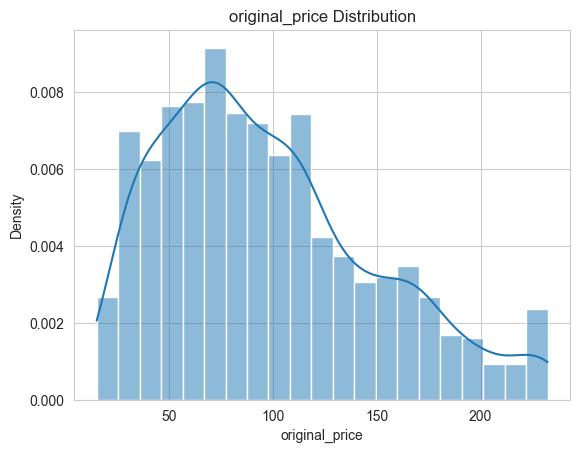
\includegraphics[width=\linewidth]{output/plots/original_price_hist.png}%
\caption{Visualization: original\_price\_hist.png}%
\end{figure}

%
\end{minipage}%
\begin{minipage}[c]{0.48\textwidth}%


\begin{figure}[H]%
\centering%
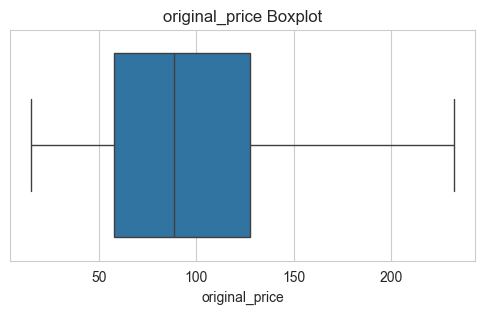
\includegraphics[width=\linewidth]{output/plots/original_price_box.png}%
\caption{Visualization: original\_price\_box.png}%
\end{figure}

%
\end{minipage}%
\vspace{10pt}%
\\%
\begin{minipage}[c]{0.48\textwidth}%


\begin{figure}[H]%
\centering%
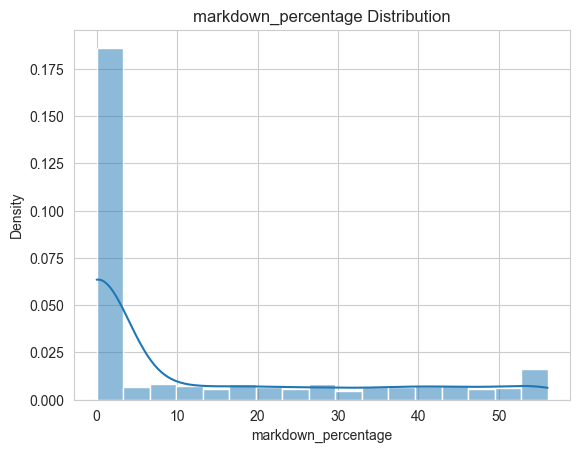
\includegraphics[width=\linewidth]{output/plots/markdown_percentage_hist.png}%
\caption{Visualization: markdown\_percentage\_hist.png}%
\end{figure}

%
\end{minipage}%
\begin{minipage}[c]{0.48\textwidth}%


\begin{figure}[H]%
\centering%
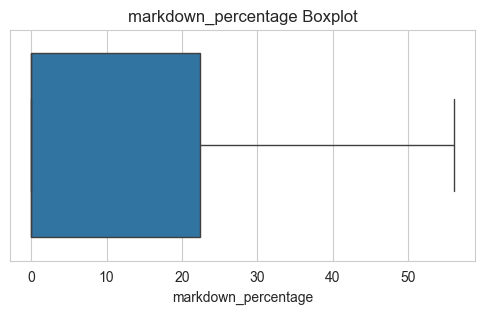
\includegraphics[width=\linewidth]{output/plots/markdown_percentage_box.png}%
\caption{Visualization: markdown\_percentage\_box.png}%
\end{figure}

%
\end{minipage}%
\vspace{10pt}%
\\%
\begin{minipage}[c]{0.48\textwidth}%


\begin{figure}[H]%
\centering%
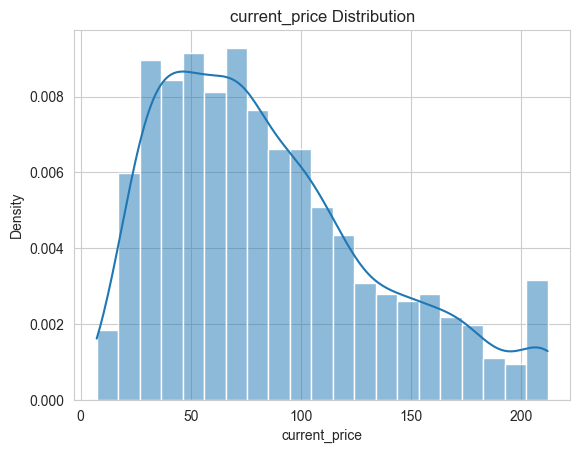
\includegraphics[width=\linewidth]{output/plots/current_price_hist.png}%
\caption{Visualization: current\_price\_hist.png}%
\end{figure}

%
\end{minipage}%
\begin{minipage}[c]{0.48\textwidth}%


\begin{figure}[H]%
\centering%
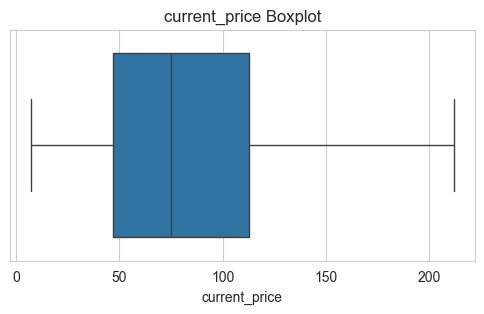
\includegraphics[width=\linewidth]{output/plots/current_price_box.png}%
\caption{Visualization: current\_price\_box.png}%
\end{figure}

%
\end{minipage}%
\vspace{10pt}%
\\%
\begin{minipage}[c]{0.48\textwidth}%


\begin{figure}[H]%
\centering%
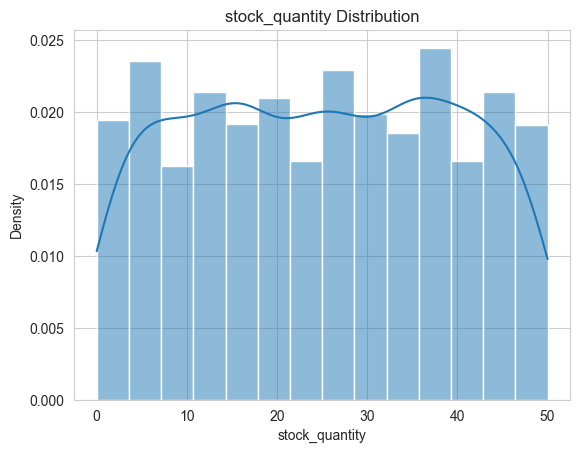
\includegraphics[width=\linewidth]{output/plots/stock_quantity_hist.png}%
\caption{Visualization: stock\_quantity\_hist.png}%
\end{figure}

%
\end{minipage}%
\begin{minipage}[c]{0.48\textwidth}%


\begin{figure}[H]%
\centering%
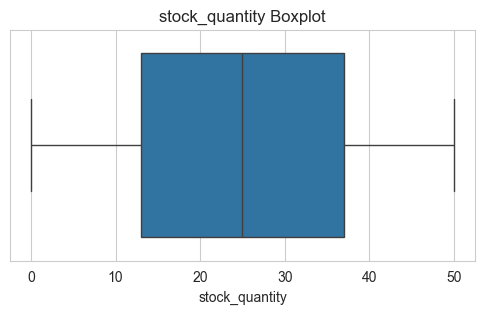
\includegraphics[width=\linewidth]{output/plots/stock_quantity_box.png}%
\caption{Visualization: stock\_quantity\_box.png}%
\end{figure}

%
\end{minipage}%
\vspace{10pt}%
\\%
\begin{minipage}[c]{0.48\textwidth}%


\begin{figure}[H]%
\centering%
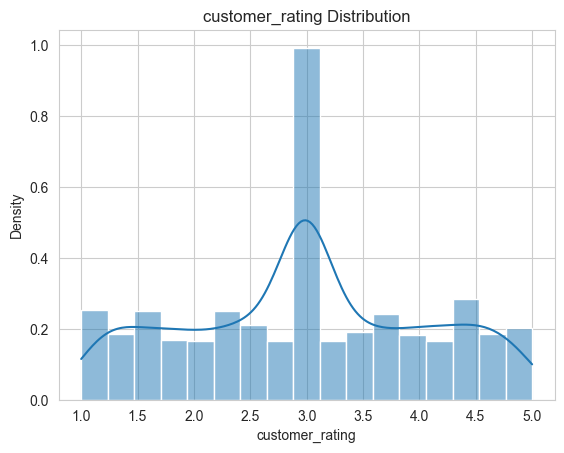
\includegraphics[width=\linewidth]{output/plots/customer_rating_hist.png}%
\caption{Visualization: customer\_rating\_hist.png}%
\end{figure}

%
\end{minipage}%
\begin{minipage}[c]{0.48\textwidth}%


\begin{figure}[H]%
\centering%
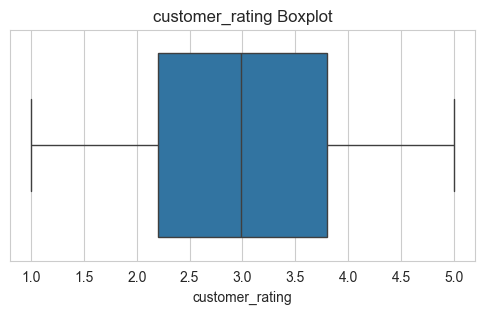
\includegraphics[width=\linewidth]{output/plots/customer_rating_box.png}%
\caption{Visualization: customer\_rating\_box.png}%
\end{figure}

%
\end{minipage}%
\vspace{10pt}%
\\%
\begin{minipage}[c]{0.48\textwidth}%


\begin{figure}[H]%
\centering%
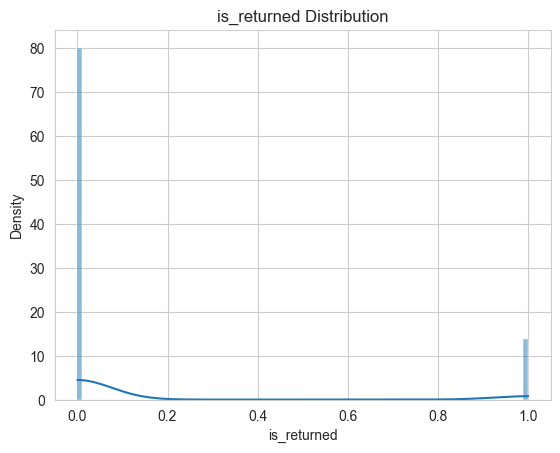
\includegraphics[width=\linewidth]{output/plots/is_returned_hist.png}%
\caption{Visualization: is\_returned\_hist.png}%
\end{figure}

%
\end{minipage}%
\begin{minipage}[c]{0.48\textwidth}%


\begin{figure}[H]%
\centering%
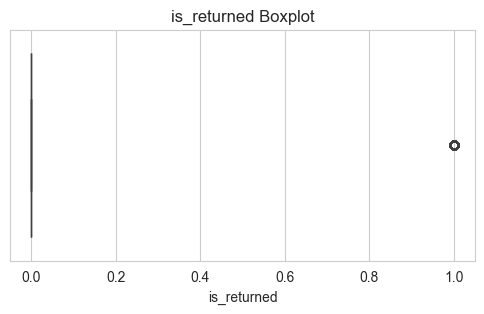
\includegraphics[width=\linewidth]{output/plots/is_returned_box.png}%
\caption{Visualization: is\_returned\_box.png}%
\end{figure}

%
\end{minipage}%
\vspace{10pt}%
\\%
\begin{minipage}[c]{0.48\textwidth}%


\begin{figure}[H]%
\centering%
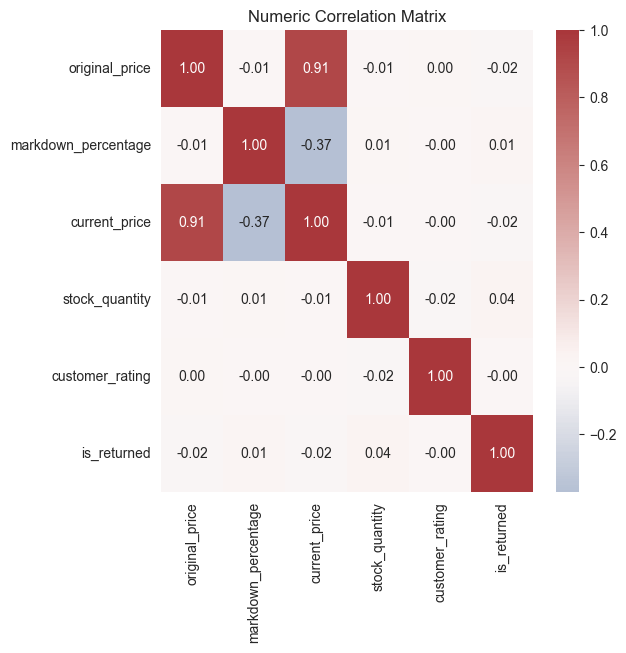
\includegraphics[width=\linewidth]{output/plots/correlation_heatmap.png}%
\caption{Visualization: correlation\_heatmap.png}%
\end{figure}

%
\end{minipage}%
\begin{minipage}[c]{0.48\textwidth}%


\begin{figure}[H]%
\centering%
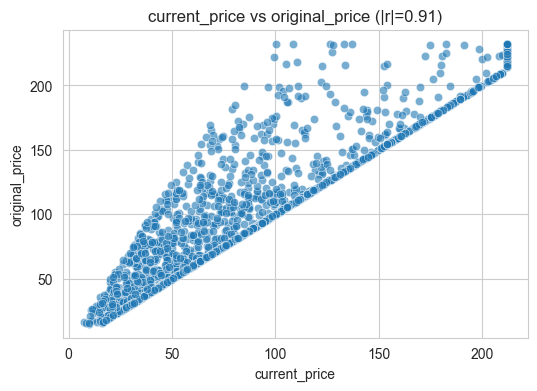
\includegraphics[width=\linewidth]{output/plots/current_price_vs_original_price_scatter.png}%
\caption{Visualization: current\_price\_vs\_original\_price\_scatter.png}%
\end{figure}

%
\end{minipage}%
\vspace{10pt}%
\\%
\begin{minipage}[c]{0.48\textwidth}%


\begin{figure}[H]%
\centering%
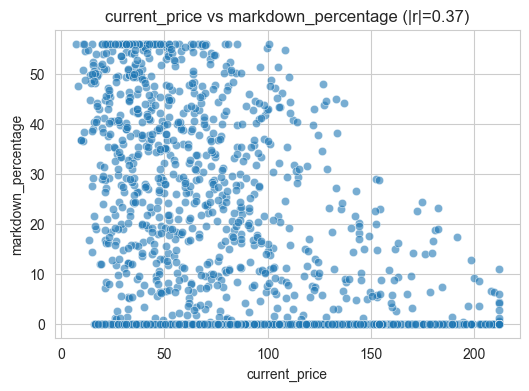
\includegraphics[width=\linewidth]{output/plots/current_price_vs_markdown_percentage_scatter.png}%
\caption{Visualization: current\_price\_vs\_markdown\_percentage\_scatter.png}%
\end{figure}

%
\end{minipage}%
\begin{minipage}[c]{0.48\textwidth}%


\begin{figure}[H]%
\centering%
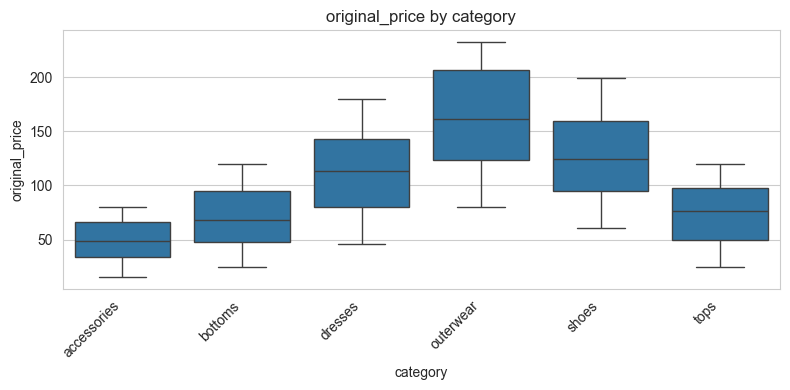
\includegraphics[width=\linewidth]{output/plots/original_price_by_category_box.png}%
\caption{Visualization: original\_price\_by\_category\_box.png}%
\end{figure}

%
\end{minipage}%
\vspace{10pt}%
\\%
\begin{minipage}[c]{0.48\textwidth}%


\begin{figure}[H]%
\centering%
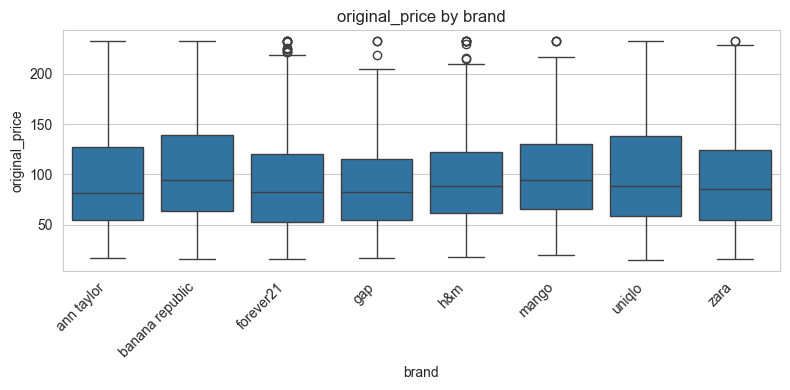
\includegraphics[width=\linewidth]{output/plots/original_price_by_brand_box.png}%
\caption{Visualization: original\_price\_by\_brand\_box.png}%
\end{figure}

%
\end{minipage}%
\begin{minipage}[c]{0.48\textwidth}%


\begin{figure}[H]%
\centering%
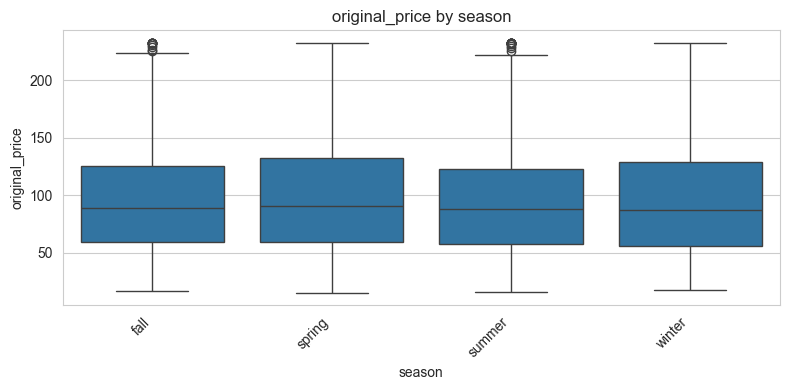
\includegraphics[width=\linewidth]{output/plots/original_price_by_season_box.png}%
\caption{Visualization: original\_price\_by\_season\_box.png}%
\end{figure}

%
\end{minipage}%
\vspace{10pt}%
\\%
\begin{minipage}[c]{0.48\textwidth}%


\begin{figure}[H]%
\centering%
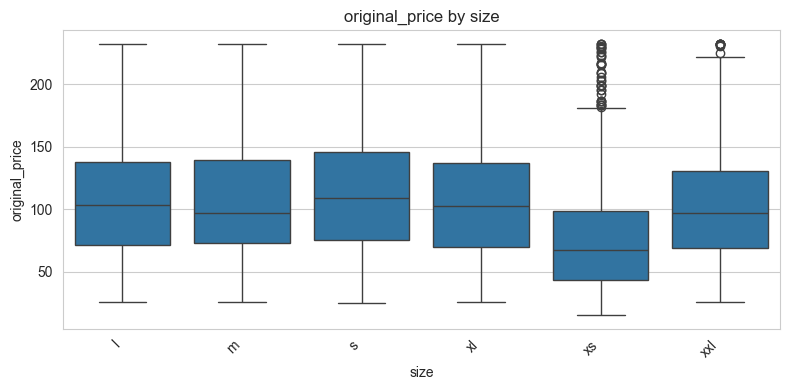
\includegraphics[width=\linewidth]{output/plots/original_price_by_size_box.png}%
\caption{Visualization: original\_price\_by\_size\_box.png}%
\end{figure}

%
\end{minipage}%
\begin{minipage}[c]{0.48\textwidth}%


\begin{figure}[H]%
\centering%
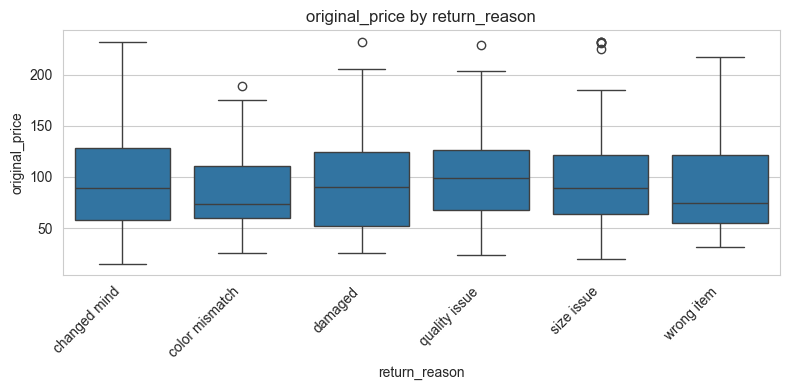
\includegraphics[width=\linewidth]{output/plots/original_price_by_return_reason_box.png}%
\caption{Visualization: original\_price\_by\_return\_reason\_box.png}%
\end{figure}

%
\end{minipage}%
\vspace{10pt}%
\\%
\begin{minipage}[c]{0.48\textwidth}%


\begin{figure}[H]%
\centering%
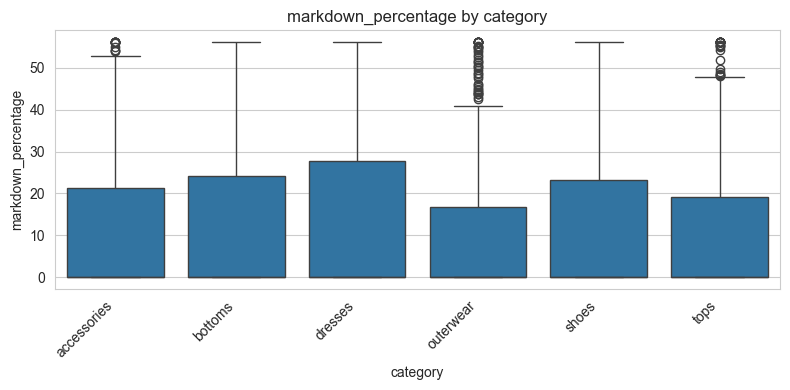
\includegraphics[width=\linewidth]{output/plots/markdown_percentage_by_category_box.png}%
\caption{Visualization: markdown\_percentage\_by\_category\_box.png}%
\end{figure}

%
\end{minipage}%
\begin{minipage}[c]{0.48\textwidth}%


\begin{figure}[H]%
\centering%
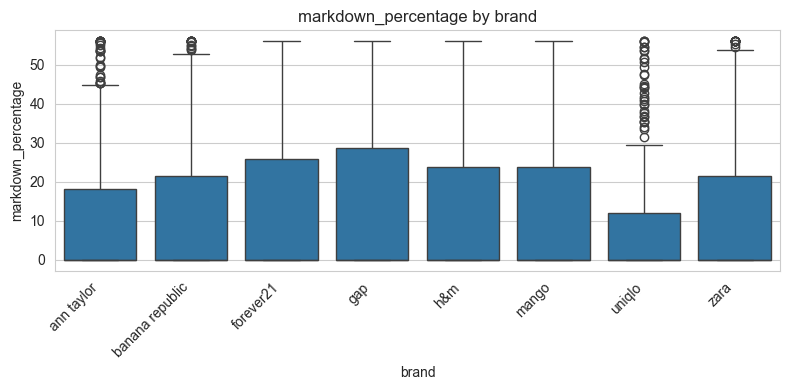
\includegraphics[width=\linewidth]{output/plots/markdown_percentage_by_brand_box.png}%
\caption{Visualization: markdown\_percentage\_by\_brand\_box.png}%
\end{figure}

%
\end{minipage}%
\vspace{10pt}%
\\%
\begin{minipage}[c]{0.48\textwidth}%


\begin{figure}[H]%
\centering%
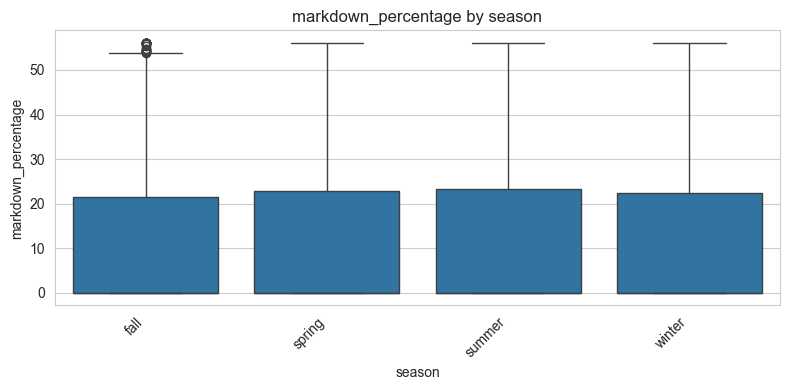
\includegraphics[width=\linewidth]{output/plots/markdown_percentage_by_season_box.png}%
\caption{Visualization: markdown\_percentage\_by\_season\_box.png}%
\end{figure}

%
\end{minipage}%
\begin{minipage}[c]{0.48\textwidth}%


\begin{figure}[H]%
\centering%
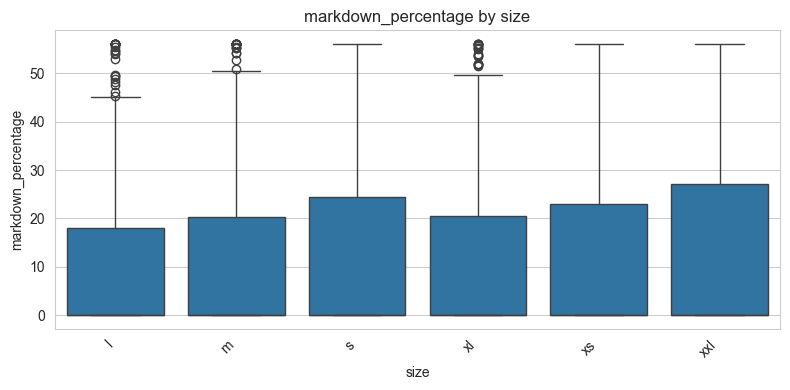
\includegraphics[width=\linewidth]{output/plots/markdown_percentage_by_size_box.png}%
\caption{Visualization: markdown\_percentage\_by\_size\_box.png}%
\end{figure}

%
\end{minipage}%
\vspace{10pt}%
\\%
\begin{minipage}[c]{0.48\textwidth}%


\begin{figure}[H]%
\centering%
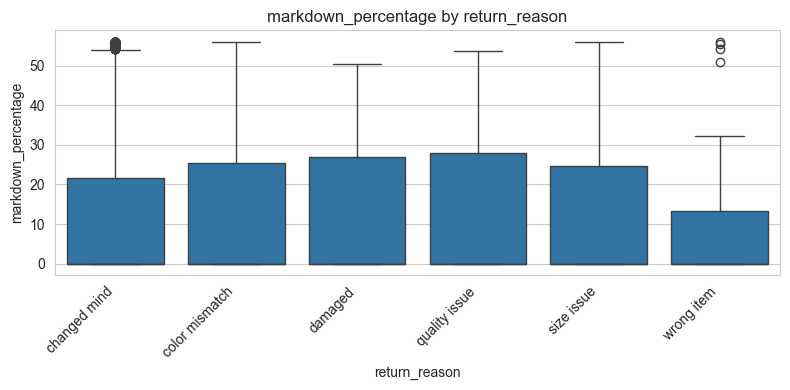
\includegraphics[width=\linewidth]{output/plots/markdown_percentage_by_return_reason_box.png}%
\caption{Visualization: markdown\_percentage\_by\_return\_reason\_box.png}%
\end{figure}

%
\end{minipage}%
\begin{minipage}[c]{0.48\textwidth}%


\begin{figure}[H]%
\centering%
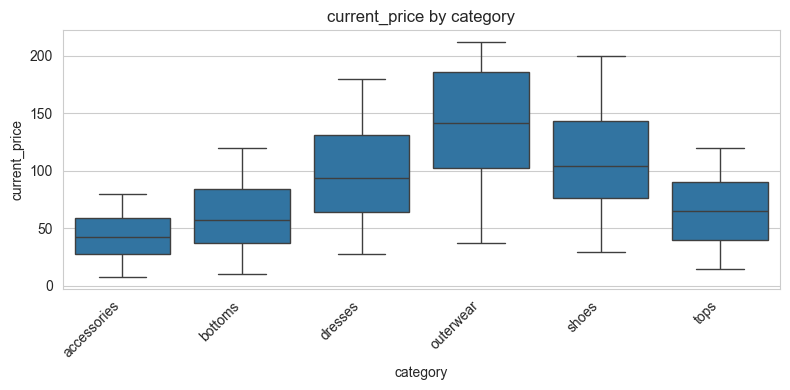
\includegraphics[width=\linewidth]{output/plots/current_price_by_category_box.png}%
\caption{Visualization: current\_price\_by\_category\_box.png}%
\end{figure}

%
\end{minipage}%
\vspace{10pt}%
\\%
\begin{minipage}[c]{0.48\textwidth}%


\begin{figure}[H]%
\centering%
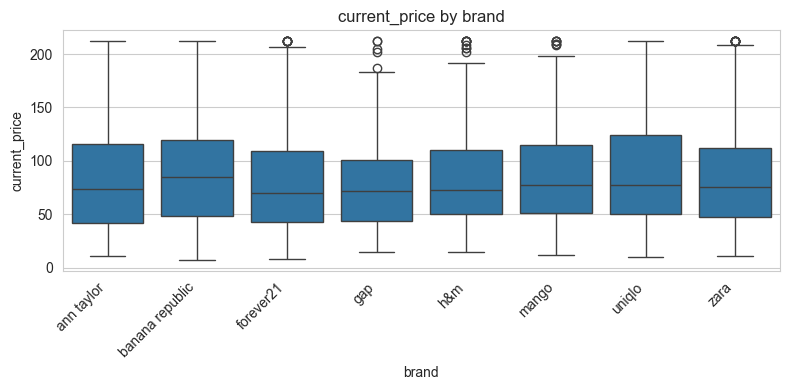
\includegraphics[width=\linewidth]{output/plots/current_price_by_brand_box.png}%
\caption{Visualization: current\_price\_by\_brand\_box.png}%
\end{figure}

%
\end{minipage}%
\begin{minipage}[c]{0.48\textwidth}%


\begin{figure}[H]%
\centering%
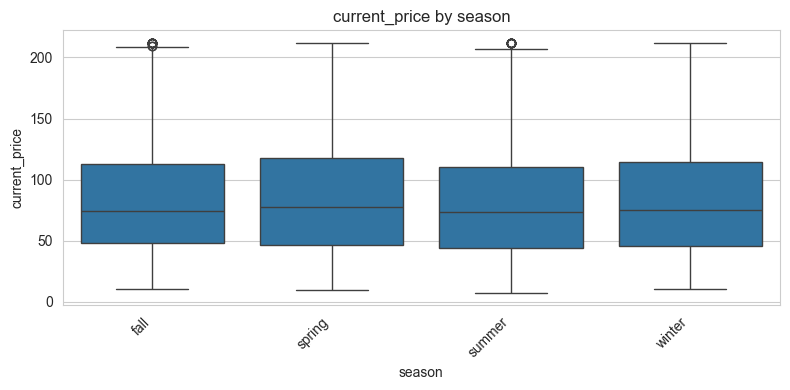
\includegraphics[width=\linewidth]{output/plots/current_price_by_season_box.png}%
\caption{Visualization: current\_price\_by\_season\_box.png}%
\end{figure}

%
\end{minipage}%
\vspace{10pt}%
\\%
\begin{minipage}[c]{0.48\textwidth}%


\begin{figure}[H]%
\centering%
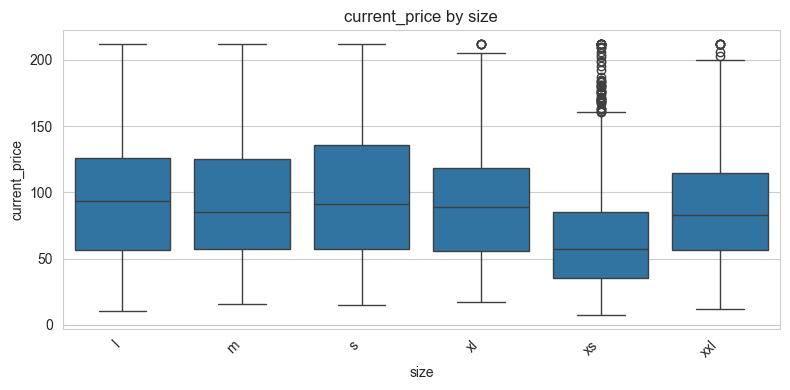
\includegraphics[width=\linewidth]{output/plots/current_price_by_size_box.png}%
\caption{Visualization: current\_price\_by\_size\_box.png}%
\end{figure}

%
\end{minipage}%
\begin{minipage}[c]{0.48\textwidth}%


\begin{figure}[H]%
\centering%
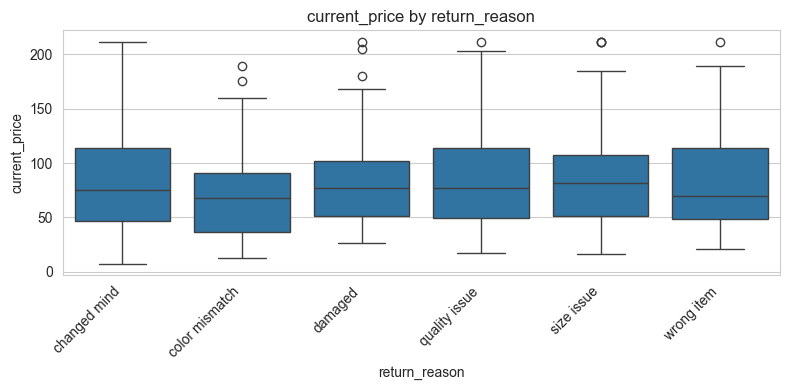
\includegraphics[width=\linewidth]{output/plots/current_price_by_return_reason_box.png}%
\caption{Visualization: current\_price\_by\_return\_reason\_box.png}%
\end{figure}

%
\end{minipage}%
\vspace{10pt}%
\\%
\begin{minipage}[c]{0.48\textwidth}%


\begin{figure}[H]%
\centering%
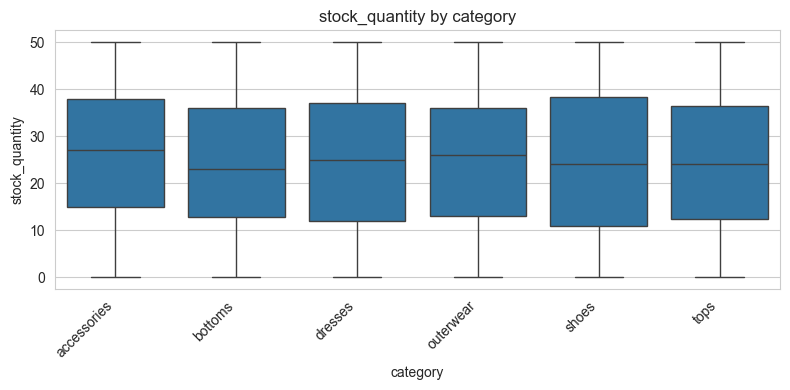
\includegraphics[width=\linewidth]{output/plots/stock_quantity_by_category_box.png}%
\caption{Visualization: stock\_quantity\_by\_category\_box.png}%
\end{figure}

%
\end{minipage}%
\begin{minipage}[c]{0.48\textwidth}%


\begin{figure}[H]%
\centering%
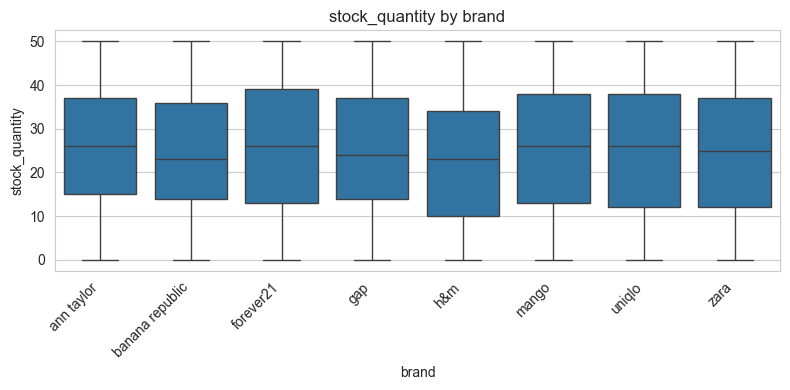
\includegraphics[width=\linewidth]{output/plots/stock_quantity_by_brand_box.png}%
\caption{Visualization: stock\_quantity\_by\_brand\_box.png}%
\end{figure}

%
\end{minipage}%
\vspace{10pt}%
\\%
\begin{minipage}[c]{0.48\textwidth}%


\begin{figure}[H]%
\centering%
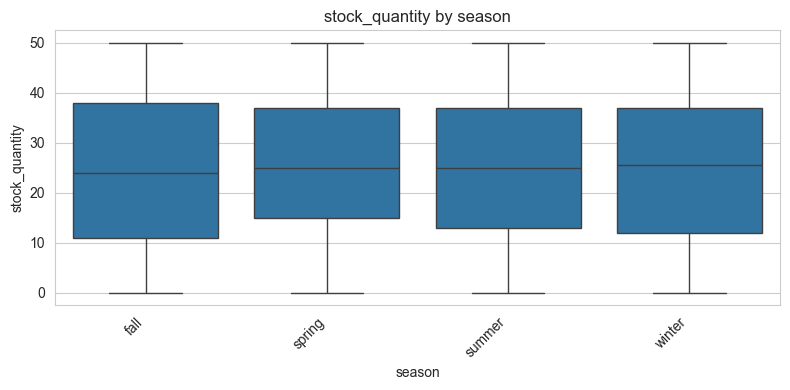
\includegraphics[width=\linewidth]{output/plots/stock_quantity_by_season_box.png}%
\caption{Visualization: stock\_quantity\_by\_season\_box.png}%
\end{figure}

%
\end{minipage}%
\begin{minipage}[c]{0.48\textwidth}%


\begin{figure}[H]%
\centering%
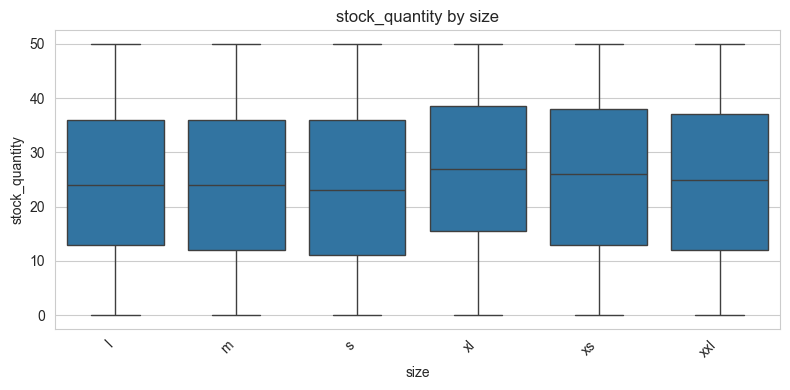
\includegraphics[width=\linewidth]{output/plots/stock_quantity_by_size_box.png}%
\caption{Visualization: stock\_quantity\_by\_size\_box.png}%
\end{figure}

%
\end{minipage}%
\vspace{10pt}%
\\%
\begin{minipage}[c]{0.48\textwidth}%


\begin{figure}[H]%
\centering%
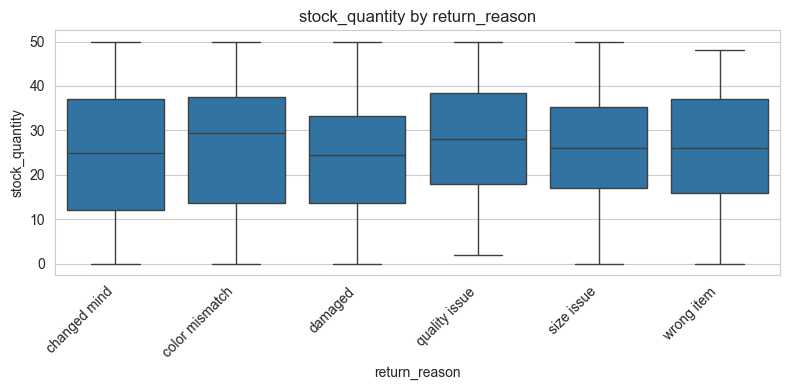
\includegraphics[width=\linewidth]{output/plots/stock_quantity_by_return_reason_box.png}%
\caption{Visualization: stock\_quantity\_by\_return\_reason\_box.png}%
\end{figure}

%
\end{minipage}%
\begin{minipage}[c]{0.48\textwidth}%


\begin{figure}[H]%
\centering%
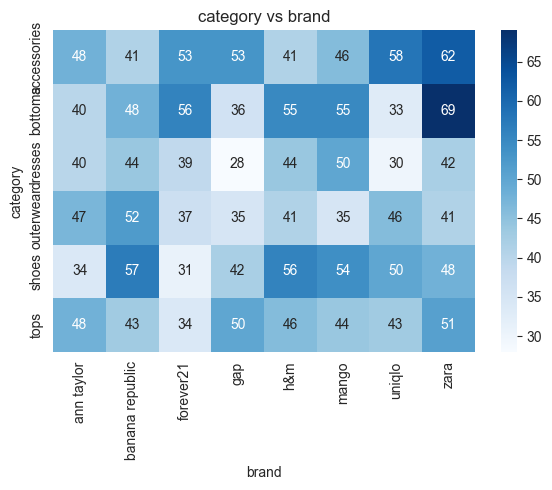
\includegraphics[width=\linewidth]{output/plots/category_vs_brand_heatmap.png}%
\caption{Visualization: category\_vs\_brand\_heatmap.png}%
\end{figure}

%
\end{minipage}%
\vspace{10pt}%
\\%
\begin{minipage}[c]{0.48\textwidth}%


\begin{figure}[H]%
\centering%
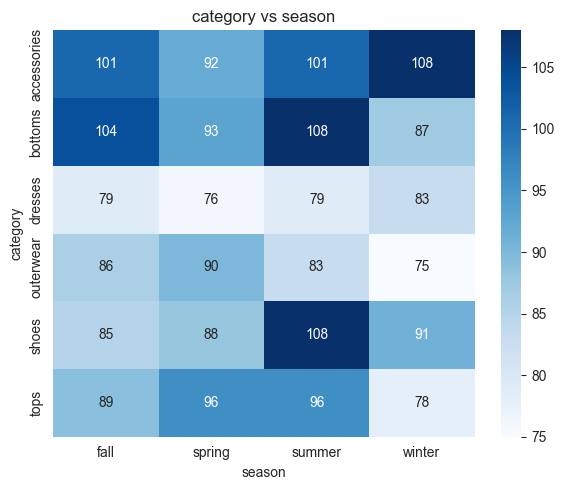
\includegraphics[width=\linewidth]{output/plots/category_vs_season_heatmap.png}%
\caption{Visualization: category\_vs\_season\_heatmap.png}%
\end{figure}

%
\end{minipage}%
\begin{minipage}[c]{0.48\textwidth}%


\begin{figure}[H]%
\centering%
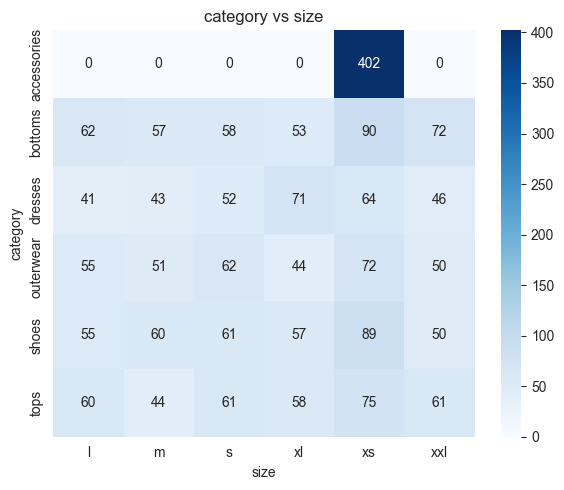
\includegraphics[width=\linewidth]{output/plots/category_vs_size_heatmap.png}%
\caption{Visualization: category\_vs\_size\_heatmap.png}%
\end{figure}

%
\end{minipage}%
\vspace{10pt}%
\\%
\begin{minipage}[c]{0.48\textwidth}%


\begin{figure}[H]%
\centering%
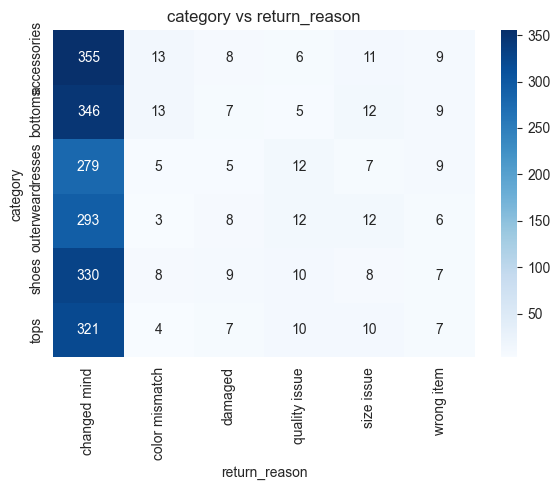
\includegraphics[width=\linewidth]{output/plots/category_vs_return_reason_heatmap.png}%
\caption{Visualization: category\_vs\_return\_reason\_heatmap.png}%
\end{figure}

%
\end{minipage}%
\begin{minipage}[c]{0.48\textwidth}%


\begin{figure}[H]%
\centering%
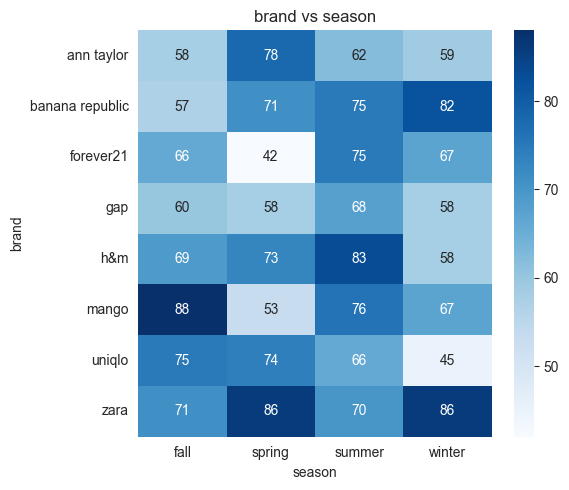
\includegraphics[width=\linewidth]{output/plots/brand_vs_season_heatmap.png}%
\caption{Visualization: brand\_vs\_season\_heatmap.png}%
\end{figure}

%
\end{minipage}%
\vspace{10pt}%
\\%
\begin{minipage}[c]{0.48\textwidth}%


\begin{figure}[H]%
\centering%
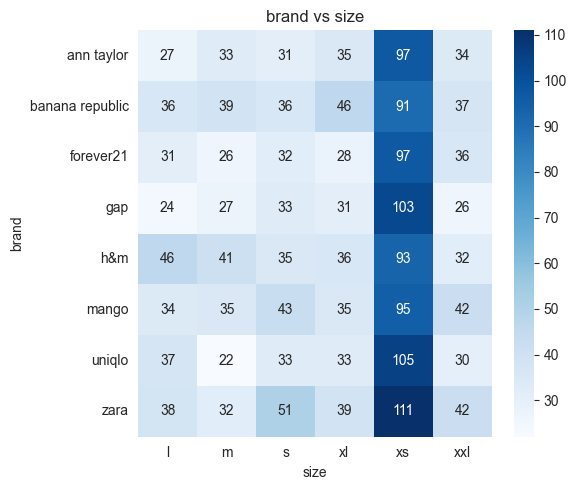
\includegraphics[width=\linewidth]{output/plots/brand_vs_size_heatmap.png}%
\caption{Visualization: brand\_vs\_size\_heatmap.png}%
\end{figure}

%
\end{minipage}%
\begin{minipage}[c]{0.48\textwidth}%


\begin{figure}[H]%
\centering%
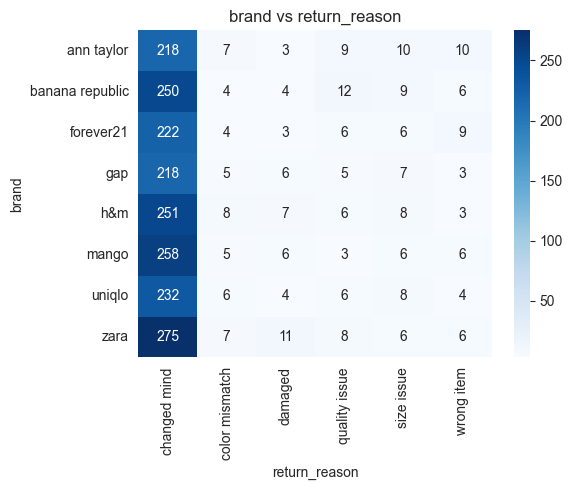
\includegraphics[width=\linewidth]{output/plots/brand_vs_return_reason_heatmap.png}%
\caption{Visualization: brand\_vs\_return\_reason\_heatmap.png}%
\end{figure}

%
\end{minipage}%
\vspace{10pt}%
\\%
\begin{minipage}[c]{0.48\textwidth}%


\begin{figure}[H]%
\centering%
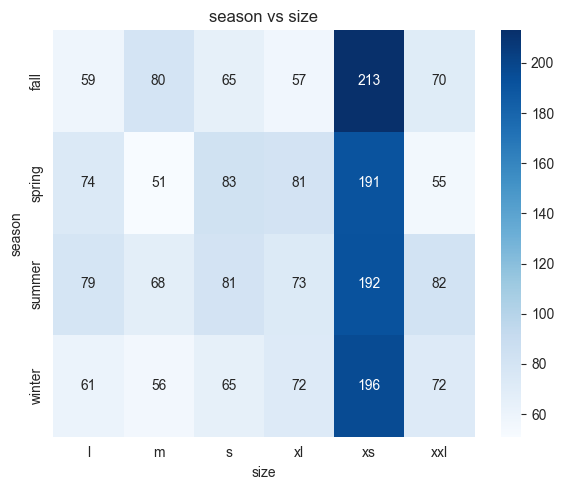
\includegraphics[width=\linewidth]{output/plots/season_vs_size_heatmap.png}%
\caption{Visualization: season\_vs\_size\_heatmap.png}%
\end{figure}

%
\end{minipage}%
\begin{minipage}[c]{0.48\textwidth}%


\begin{figure}[H]%
\centering%
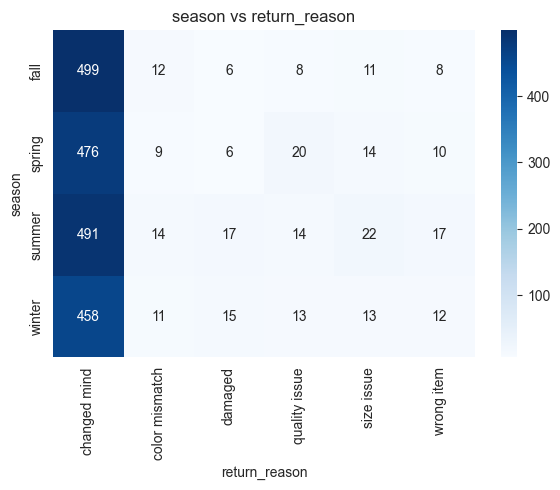
\includegraphics[width=\linewidth]{output/plots/season_vs_return_reason_heatmap.png}%
\caption{Visualization: season\_vs\_return\_reason\_heatmap.png}%
\end{figure}

%
\end{minipage}%
\vspace{10pt}%
\\%
\begin{minipage}[c]{0.48\textwidth}%


\begin{figure}[H]%
\centering%
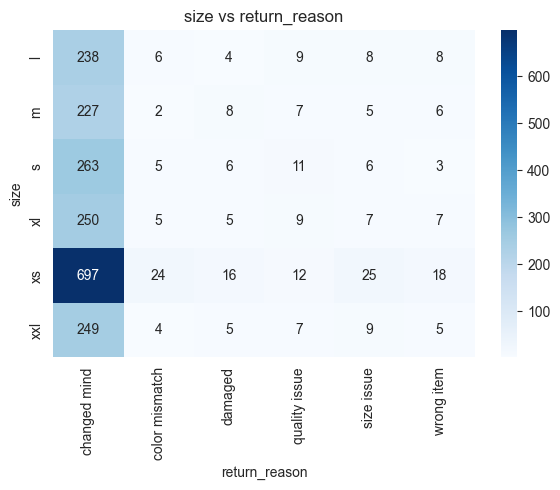
\includegraphics[width=\linewidth]{output/plots/size_vs_return_reason_heatmap.png}%
\caption{Visualization: size\_vs\_return\_reason\_heatmap.png}%
\end{figure}

%
\end{minipage}%
\begin{minipage}[c]{0.48\textwidth}%


\begin{figure}[H]%
\centering%
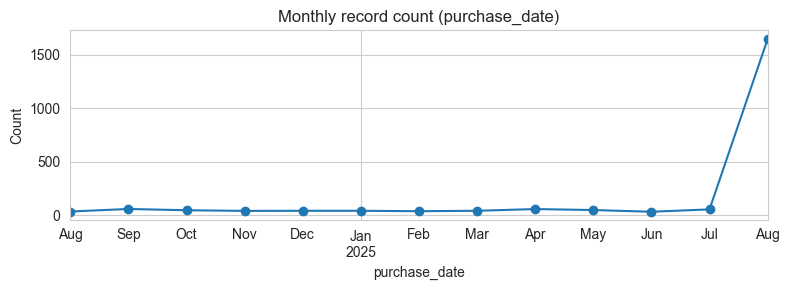
\includegraphics[width=\linewidth]{output/plots/purchase_date_monthly_count.png}%
\caption{Visualization: purchase\_date\_monthly\_count.png}%
\end{figure}

%
\end{minipage}%
\vspace{10pt}%
\\%
\begin{minipage}[c]{0.48\textwidth}%


\begin{figure}[H]%
\centering%
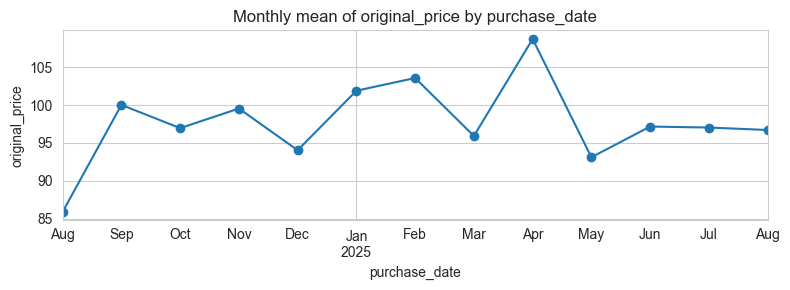
\includegraphics[width=\linewidth]{output/plots/original_price_monthly_mean_by_purchase_date.png}%
\caption{Visualization: original\_price\_monthly\_mean\_by\_purchase\_date.png}%
\end{figure}

%
\end{minipage}%
\begin{minipage}[c]{0.48\textwidth}%


\begin{figure}[H]%
\centering%
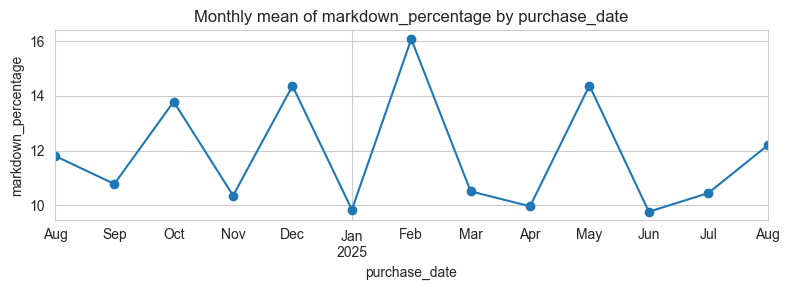
\includegraphics[width=\linewidth]{output/plots/markdown_percentage_monthly_mean_by_purchase_date.png}%
\caption{Visualization: markdown\_percentage\_monthly\_mean\_by\_purchase\_date.png}%
\end{figure}

%
\end{minipage}%
\vspace{10pt}%
\\%
\begin{minipage}[c]{0.48\textwidth}%


\begin{figure}[H]%
\centering%
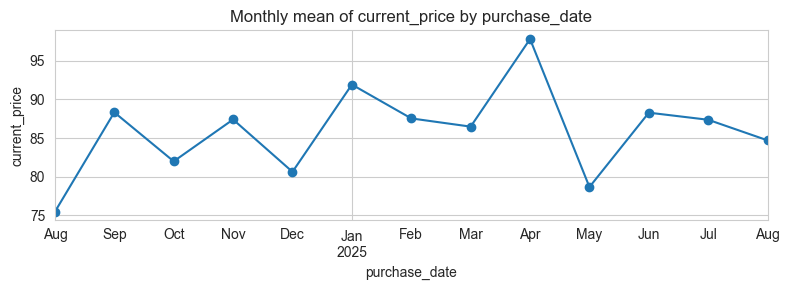
\includegraphics[width=\linewidth]{output/plots/current_price_monthly_mean_by_purchase_date.png}%
\caption{Visualization: current\_price\_monthly\_mean\_by\_purchase\_date.png}%
\end{figure}

%
\end{minipage}%
\vspace{10pt}%
\\

%
\section{Hypothesis Testing Results}%
\label{sec:HypothesisTestingResults}%
\subsection{Does the strong Spearman correlation (r=0.91) between 'original\_price' and 'current\_price' indicate potential causal or confounding factors worth testing?}%
\label{subsec:DoesthestrongSpearmancorrelation(r=0.91)betweenoriginalpriceandcurrentpriceindicatepotentialcausalorconfoundingfactorsworthtesting?}%
Test: Spearman Correlation\newline%
H₀: H₀: There is no correlation between 'original\_price' and 'current\_price'.\newline%
H₁: H₁: There is a correlation between 'original\_price' and 'current\_price'.\newline%
Conclusion: N/A

%
\subsection{Does the moderate Spearman correlation (r={-}0.36) between 'markdown\_percentage' and 'current\_price' indicate potential causal or confounding factors worth testing?}%
\label{subsec:DoesthemoderateSpearmancorrelation(r={-}0.36)betweenmarkdownpercentageandcurrentpriceindicatepotentialcausalorconfoundingfactorsworthtesting?}%
Test: Spearman Correlation\newline%
H₀: H₀: There is no correlation between 'markdown\_percentage' and 'current\_price'.\newline%
H₁: H₁: There is a correlation between 'markdown\_percentage' and 'current\_price'.\newline%
Conclusion: N/A

%
\subsection{Do different 'category' categories show significant differences in 'original\_price' means (t{-}test/ANOVA) or medians (Kruskal{-}Wallis) depending on normality?}%
\label{subsec:Dodifferentcategorycategoriesshowsignificantdifferencesinoriginalpricemeans(t{-}test/ANOVA)ormedians(Kruskal{-}Wallis)dependingonnormality?}%
Test: KRUSKAL\newline%
H₀: H₀: The distribution of 'original\_price' is the same across all groups in 'category'.\newline%
H₁: H₁: At least one group distribution of 'original\_price' in 'category' is different.\newline%
Conclusion: N/A

%
\subsection{Do different 'category' categories show significant differences in 'markdown\_percentage' means (t{-}test/ANOVA) or medians (Kruskal{-}Wallis) depending on normality?}%
\label{subsec:Dodifferentcategorycategoriesshowsignificantdifferencesinmarkdownpercentagemeans(t{-}test/ANOVA)ormedians(Kruskal{-}Wallis)dependingonnormality?}%
Test: KRUSKAL\newline%
H₀: H₀: The distribution of 'markdown\_percentage' is the same across all groups in 'category'.\newline%
H₁: H₁: At least one group distribution of 'markdown\_percentage' in 'category' is different.\newline%
Conclusion: N/A

%
\subsection{Do different 'category' categories show significant differences in 'current\_price' means (t{-}test/ANOVA) or medians (Kruskal{-}Wallis) depending on normality?}%
\label{subsec:Dodifferentcategorycategoriesshowsignificantdifferencesincurrentpricemeans(t{-}test/ANOVA)ormedians(Kruskal{-}Wallis)dependingonnormality?}%
Test: KRUSKAL\newline%
H₀: H₀: The distribution of 'current\_price' is the same across all groups in 'category'.\newline%
H₁: H₁: At least one group distribution of 'current\_price' in 'category' is different.\newline%
Conclusion: N/A

%
\subsection{Do different 'category' categories show significant differences in 'stock\_quantity' means (t{-}test/ANOVA) or medians (Kruskal{-}Wallis) depending on normality?}%
\label{subsec:Dodifferentcategorycategoriesshowsignificantdifferencesinstockquantitymeans(t{-}test/ANOVA)ormedians(Kruskal{-}Wallis)dependingonnormality?}%
Test: KRUSKAL\newline%
H₀: H₀: The distribution of 'stock\_quantity' is the same across all groups in 'category'.\newline%
H₁: H₁: At least one group distribution of 'stock\_quantity' in 'category' is different.\newline%
Conclusion: N/A

%
\subsection{Do different 'category' categories show significant differences in 'customer\_rating' means (t{-}test/ANOVA) or medians (Kruskal{-}Wallis) depending on normality?}%
\label{subsec:Dodifferentcategorycategoriesshowsignificantdifferencesincustomerratingmeans(t{-}test/ANOVA)ormedians(Kruskal{-}Wallis)dependingonnormality?}%
Test: KRUSKAL\newline%
H₀: H₀: The distribution of 'customer\_rating' is the same across all groups in 'category'.\newline%
H₁: H₁: At least one group distribution of 'customer\_rating' in 'category' is different.\newline%
Conclusion: N/A

%
\subsection{Do different 'brand' categories show significant differences in 'original\_price' means (t{-}test/ANOVA) or medians (Kruskal{-}Wallis) depending on normality?}%
\label{subsec:Dodifferentbrandcategoriesshowsignificantdifferencesinoriginalpricemeans(t{-}test/ANOVA)ormedians(Kruskal{-}Wallis)dependingonnormality?}%
Test: KRUSKAL\newline%
H₀: H₀: The distribution of 'original\_price' is the same across all groups in 'brand'.\newline%
H₁: H₁: At least one group distribution of 'original\_price' in 'brand' is different.\newline%
Conclusion: N/A

%
\subsection{Do different 'brand' categories show significant differences in 'markdown\_percentage' means (t{-}test/ANOVA) or medians (Kruskal{-}Wallis) depending on normality?}%
\label{subsec:Dodifferentbrandcategoriesshowsignificantdifferencesinmarkdownpercentagemeans(t{-}test/ANOVA)ormedians(Kruskal{-}Wallis)dependingonnormality?}%
Test: KRUSKAL\newline%
H₀: H₀: The distribution of 'markdown\_percentage' is the same across all groups in 'brand'.\newline%
H₁: H₁: At least one group distribution of 'markdown\_percentage' in 'brand' is different.\newline%
Conclusion: N/A

%
\subsection{Do different 'brand' categories show significant differences in 'current\_price' means (t{-}test/ANOVA) or medians (Kruskal{-}Wallis) depending on normality?}%
\label{subsec:Dodifferentbrandcategoriesshowsignificantdifferencesincurrentpricemeans(t{-}test/ANOVA)ormedians(Kruskal{-}Wallis)dependingonnormality?}%
Test: KRUSKAL\newline%
H₀: H₀: The distribution of 'current\_price' is the same across all groups in 'brand'.\newline%
H₁: H₁: At least one group distribution of 'current\_price' in 'brand' is different.\newline%
Conclusion: N/A

%
\subsection{Do different 'brand' categories show significant differences in 'stock\_quantity' means (t{-}test/ANOVA) or medians (Kruskal{-}Wallis) depending on normality?}%
\label{subsec:Dodifferentbrandcategoriesshowsignificantdifferencesinstockquantitymeans(t{-}test/ANOVA)ormedians(Kruskal{-}Wallis)dependingonnormality?}%
Test: KRUSKAL\newline%
H₀: H₀: The distribution of 'stock\_quantity' is the same across all groups in 'brand'.\newline%
H₁: H₁: At least one group distribution of 'stock\_quantity' in 'brand' is different.\newline%
Conclusion: N/A

%
\subsection{Do different 'brand' categories show significant differences in 'customer\_rating' means (t{-}test/ANOVA) or medians (Kruskal{-}Wallis) depending on normality?}%
\label{subsec:Dodifferentbrandcategoriesshowsignificantdifferencesincustomerratingmeans(t{-}test/ANOVA)ormedians(Kruskal{-}Wallis)dependingonnormality?}%
Test: KRUSKAL\newline%
H₀: H₀: The distribution of 'customer\_rating' is the same across all groups in 'brand'.\newline%
H₁: H₁: At least one group distribution of 'customer\_rating' in 'brand' is different.\newline%
Conclusion: N/A

%
\subsection{Do different 'season' categories show significant differences in 'original\_price' means (t{-}test/ANOVA) or medians (Kruskal{-}Wallis) depending on normality?}%
\label{subsec:Dodifferentseasoncategoriesshowsignificantdifferencesinoriginalpricemeans(t{-}test/ANOVA)ormedians(Kruskal{-}Wallis)dependingonnormality?}%
Test: KRUSKAL\newline%
H₀: H₀: The distribution of 'original\_price' is the same across all groups in 'season'.\newline%
H₁: H₁: At least one group distribution of 'original\_price' in 'season' is different.\newline%
Conclusion: N/A

%
\subsection{Do different 'season' categories show significant differences in 'markdown\_percentage' means (t{-}test/ANOVA) or medians (Kruskal{-}Wallis) depending on normality?}%
\label{subsec:Dodifferentseasoncategoriesshowsignificantdifferencesinmarkdownpercentagemeans(t{-}test/ANOVA)ormedians(Kruskal{-}Wallis)dependingonnormality?}%
Test: KRUSKAL\newline%
H₀: H₀: The distribution of 'markdown\_percentage' is the same across all groups in 'season'.\newline%
H₁: H₁: At least one group distribution of 'markdown\_percentage' in 'season' is different.\newline%
Conclusion: N/A

%
\subsection{Do different 'season' categories show significant differences in 'current\_price' means (t{-}test/ANOVA) or medians (Kruskal{-}Wallis) depending on normality?}%
\label{subsec:Dodifferentseasoncategoriesshowsignificantdifferencesincurrentpricemeans(t{-}test/ANOVA)ormedians(Kruskal{-}Wallis)dependingonnormality?}%
Test: KRUSKAL\newline%
H₀: H₀: The distribution of 'current\_price' is the same across all groups in 'season'.\newline%
H₁: H₁: At least one group distribution of 'current\_price' in 'season' is different.\newline%
Conclusion: N/A

%
\subsection{Do different 'season' categories show significant differences in 'stock\_quantity' means (t{-}test/ANOVA) or medians (Kruskal{-}Wallis) depending on normality?}%
\label{subsec:Dodifferentseasoncategoriesshowsignificantdifferencesinstockquantitymeans(t{-}test/ANOVA)ormedians(Kruskal{-}Wallis)dependingonnormality?}%
Test: KRUSKAL\newline%
H₀: H₀: The distribution of 'stock\_quantity' is the same across all groups in 'season'.\newline%
H₁: H₁: At least one group distribution of 'stock\_quantity' in 'season' is different.\newline%
Conclusion: N/A

%
\subsection{Do different 'season' categories show significant differences in 'customer\_rating' means (t{-}test/ANOVA) or medians (Kruskal{-}Wallis) depending on normality?}%
\label{subsec:Dodifferentseasoncategoriesshowsignificantdifferencesincustomerratingmeans(t{-}test/ANOVA)ormedians(Kruskal{-}Wallis)dependingonnormality?}%
Test: KRUSKAL\newline%
H₀: H₀: The distribution of 'customer\_rating' is the same across all groups in 'season'.\newline%
H₁: H₁: At least one group distribution of 'customer\_rating' in 'season' is different.\newline%
Conclusion: N/A

%
\subsection{Do different 'size' categories show significant differences in 'original\_price' means (t{-}test/ANOVA) or medians (Kruskal{-}Wallis) depending on normality?}%
\label{subsec:Dodifferentsizecategoriesshowsignificantdifferencesinoriginalpricemeans(t{-}test/ANOVA)ormedians(Kruskal{-}Wallis)dependingonnormality?}%
Test: KRUSKAL\newline%
H₀: H₀: The distribution of 'original\_price' is the same across all groups in 'size'.\newline%
H₁: H₁: At least one group distribution of 'original\_price' in 'size' is different.\newline%
Conclusion: N/A

%
\subsection{Do different 'size' categories show significant differences in 'markdown\_percentage' means (t{-}test/ANOVA) or medians (Kruskal{-}Wallis) depending on normality?}%
\label{subsec:Dodifferentsizecategoriesshowsignificantdifferencesinmarkdownpercentagemeans(t{-}test/ANOVA)ormedians(Kruskal{-}Wallis)dependingonnormality?}%
Test: KRUSKAL\newline%
H₀: H₀: The distribution of 'markdown\_percentage' is the same across all groups in 'size'.\newline%
H₁: H₁: At least one group distribution of 'markdown\_percentage' in 'size' is different.\newline%
Conclusion: N/A

%
\subsection{Do different 'size' categories show significant differences in 'current\_price' means (t{-}test/ANOVA) or medians (Kruskal{-}Wallis) depending on normality?}%
\label{subsec:Dodifferentsizecategoriesshowsignificantdifferencesincurrentpricemeans(t{-}test/ANOVA)ormedians(Kruskal{-}Wallis)dependingonnormality?}%
Test: KRUSKAL\newline%
H₀: H₀: The distribution of 'current\_price' is the same across all groups in 'size'.\newline%
H₁: H₁: At least one group distribution of 'current\_price' in 'size' is different.\newline%
Conclusion: N/A

%
\subsection{Do different 'size' categories show significant differences in 'stock\_quantity' means (t{-}test/ANOVA) or medians (Kruskal{-}Wallis) depending on normality?}%
\label{subsec:Dodifferentsizecategoriesshowsignificantdifferencesinstockquantitymeans(t{-}test/ANOVA)ormedians(Kruskal{-}Wallis)dependingonnormality?}%
Test: KRUSKAL\newline%
H₀: H₀: The distribution of 'stock\_quantity' is the same across all groups in 'size'.\newline%
H₁: H₁: At least one group distribution of 'stock\_quantity' in 'size' is different.\newline%
Conclusion: N/A

%
\subsection{Do different 'size' categories show significant differences in 'customer\_rating' means (t{-}test/ANOVA) or medians (Kruskal{-}Wallis) depending on normality?}%
\label{subsec:Dodifferentsizecategoriesshowsignificantdifferencesincustomerratingmeans(t{-}test/ANOVA)ormedians(Kruskal{-}Wallis)dependingonnormality?}%
Test: KRUSKAL\newline%
H₀: H₀: The distribution of 'customer\_rating' is the same across all groups in 'size'.\newline%
H₁: H₁: At least one group distribution of 'customer\_rating' in 'size' is different.\newline%
Conclusion: N/A

%
\subsection{Do different 'return\_reason' categories show significant differences in 'original\_price' means (t{-}test/ANOVA) or medians (Kruskal{-}Wallis) depending on normality?}%
\label{subsec:Dodifferentreturnreasoncategoriesshowsignificantdifferencesinoriginalpricemeans(t{-}test/ANOVA)ormedians(Kruskal{-}Wallis)dependingonnormality?}%
Test: KRUSKAL\newline%
H₀: H₀: The distribution of 'original\_price' is the same across all groups in 'return\_reason'.\newline%
H₁: H₁: At least one group distribution of 'original\_price' in 'return\_reason' is different.\newline%
Conclusion: N/A

%
\subsection{Do different 'return\_reason' categories show significant differences in 'markdown\_percentage' means (t{-}test/ANOVA) or medians (Kruskal{-}Wallis) depending on normality?}%
\label{subsec:Dodifferentreturnreasoncategoriesshowsignificantdifferencesinmarkdownpercentagemeans(t{-}test/ANOVA)ormedians(Kruskal{-}Wallis)dependingonnormality?}%
Test: KRUSKAL\newline%
H₀: H₀: The distribution of 'markdown\_percentage' is the same across all groups in 'return\_reason'.\newline%
H₁: H₁: At least one group distribution of 'markdown\_percentage' in 'return\_reason' is different.\newline%
Conclusion: N/A

%
\subsection{Do different 'return\_reason' categories show significant differences in 'current\_price' means (t{-}test/ANOVA) or medians (Kruskal{-}Wallis) depending on normality?}%
\label{subsec:Dodifferentreturnreasoncategoriesshowsignificantdifferencesincurrentpricemeans(t{-}test/ANOVA)ormedians(Kruskal{-}Wallis)dependingonnormality?}%
Test: KRUSKAL\newline%
H₀: H₀: The distribution of 'current\_price' is the same across all groups in 'return\_reason'.\newline%
H₁: H₁: At least one group distribution of 'current\_price' in 'return\_reason' is different.\newline%
Conclusion: N/A

%
\subsection{Do different 'return\_reason' categories show significant differences in 'stock\_quantity' means (t{-}test/ANOVA) or medians (Kruskal{-}Wallis) depending on normality?}%
\label{subsec:Dodifferentreturnreasoncategoriesshowsignificantdifferencesinstockquantitymeans(t{-}test/ANOVA)ormedians(Kruskal{-}Wallis)dependingonnormality?}%
Test: KRUSKAL\newline%
H₀: H₀: The distribution of 'stock\_quantity' is the same across all groups in 'return\_reason'.\newline%
H₁: H₁: At least one group distribution of 'stock\_quantity' in 'return\_reason' is different.\newline%
Conclusion: N/A

%
\subsection{Do different 'return\_reason' categories show significant differences in 'customer\_rating' means (t{-}test/ANOVA) or medians (Kruskal{-}Wallis) depending on normality?}%
\label{subsec:Dodifferentreturnreasoncategoriesshowsignificantdifferencesincustomerratingmeans(t{-}test/ANOVA)ormedians(Kruskal{-}Wallis)dependingonnormality?}%
Test: KRUSKAL\newline%
H₀: H₀: The distribution of 'customer\_rating' is the same across all groups in 'return\_reason'.\newline%
H₁: H₁: At least one group distribution of 'customer\_rating' in 'return\_reason' is different.\newline%
Conclusion: N/A

%
\subsection{Is there an association between 'category' and 'brand' (Chi{-}square test with Cramér’s V effect size)?}%
\label{subsec:Isthereanassociationbetweencategoryandbrand(Chi{-}squaretestwithCramrsVeffectsize)?}%
Test: Chi{-}square\newline%
H₀: H₀: 'category' and 'brand' are independent.\newline%
H₁: H₁: 'category' and 'brand' are not independent.\newline%
Conclusion: N/A

%
\subsection{Is there an association between 'category' and 'season' (Chi{-}square test with Cramér’s V effect size)?}%
\label{subsec:Isthereanassociationbetweencategoryandseason(Chi{-}squaretestwithCramrsVeffectsize)?}%
Test: Chi{-}square\newline%
H₀: H₀: 'category' and 'season' are independent.\newline%
H₁: H₁: 'category' and 'season' are not independent.\newline%
Conclusion: N/A

%
\subsection{Is there an association between 'category' and 'size' (Chi{-}square test with Cramér’s V effect size)?}%
\label{subsec:Isthereanassociationbetweencategoryandsize(Chi{-}squaretestwithCramrsVeffectsize)?}%
Test: Chi{-}square\newline%
H₀: H₀: 'category' and 'size' are independent.\newline%
H₁: H₁: 'category' and 'size' are not independent.\newline%
Conclusion: N/A

%
\subsection{Is there an association between 'category' and 'return\_reason' (Chi{-}square test with Cramér’s V effect size)?}%
\label{subsec:Isthereanassociationbetweencategoryandreturnreason(Chi{-}squaretestwithCramrsVeffectsize)?}%
Test: Chi{-}square\newline%
H₀: H₀: 'category' and 'return\_reason' are independent.\newline%
H₁: H₁: 'category' and 'return\_reason' are not independent.\newline%
Conclusion: N/A

%
\subsection{Is there an association between 'brand' and 'season' (Chi{-}square test with Cramér’s V effect size)?}%
\label{subsec:Isthereanassociationbetweenbrandandseason(Chi{-}squaretestwithCramrsVeffectsize)?}%
Test: Chi{-}square\newline%
H₀: H₀: 'brand' and 'season' are independent.\newline%
H₁: H₁: 'brand' and 'season' are not independent.\newline%
Conclusion: N/A

%
\subsection{Is there an association between 'brand' and 'size' (Chi{-}square test with Cramér’s V effect size)?}%
\label{subsec:Isthereanassociationbetweenbrandandsize(Chi{-}squaretestwithCramrsVeffectsize)?}%
Test: Chi{-}square\newline%
H₀: H₀: 'brand' and 'size' are independent.\newline%
H₁: H₁: 'brand' and 'size' are not independent.\newline%
Conclusion: N/A

%
\subsection{Is there an association between 'brand' and 'return\_reason' (Chi{-}square test with Cramér’s V effect size)?}%
\label{subsec:Isthereanassociationbetweenbrandandreturnreason(Chi{-}squaretestwithCramrsVeffectsize)?}%
Test: Chi{-}square\newline%
H₀: H₀: 'brand' and 'return\_reason' are independent.\newline%
H₁: H₁: 'brand' and 'return\_reason' are not independent.\newline%
Conclusion: N/A

%
\subsection{Is there an association between 'season' and 'size' (Chi{-}square test with Cramér’s V effect size)?}%
\label{subsec:Isthereanassociationbetweenseasonandsize(Chi{-}squaretestwithCramrsVeffectsize)?}%
Test: Chi{-}square\newline%
H₀: H₀: 'season' and 'size' are independent.\newline%
H₁: H₁: 'season' and 'size' are not independent.\newline%
Conclusion: N/A

%
\subsection{Is there an association between 'season' and 'return\_reason' (Chi{-}square test with Cramér’s V effect size)?}%
\label{subsec:Isthereanassociationbetweenseasonandreturnreason(Chi{-}squaretestwithCramrsVeffectsize)?}%
Test: Chi{-}square\newline%
H₀: H₀: 'season' and 'return\_reason' are independent.\newline%
H₁: H₁: 'season' and 'return\_reason' are not independent.\newline%
Conclusion: N/A

%
\subsection{Is there an association between 'size' and 'return\_reason' (Chi{-}square test with Cramér’s V effect size)?}%
\label{subsec:Isthereanassociationbetweensizeandreturnreason(Chi{-}squaretestwithCramrsVeffectsize)?}%
Test: Chi{-}square\newline%
H₀: H₀: 'size' and 'return\_reason' are independent.\newline%
H₁: H₁: 'size' and 'return\_reason' are not independent.\newline%
Conclusion: N/A

%
\end{document}